\documentclass[10pt, a4paper, landscape]{article}

% ----- packages -----
\usepackage{amsmath} % AMS mathematical facilities for LaTeX
\usepackage{enumitem} % Control layout of itemize, enumerate, description
\usepackage{fancyhdr} % Extensive control of page headers and footers in LaTeX2
\usepackage{geometry} % Flexible and complete interface to document dimensions
\usepackage{graphicx} % Enhanced support for graphics
\usepackage{hyperref} % Extensive support for hypertext in LaTeX
\usepackage{multicol} % Intermix single and multiple columns
\usepackage{parskip} % Layout with zero \parindent, non-zero \parskip
\usepackage{tikz} % Create PostScript and PDF graphics in TeX
\usepackage{titlesec} % Select alternative section titles

% ----- tikz libraries -----
\usetikzlibrary{patterns}

% ----- random seed -----
\pgfmathsetseed{12}

% ----- custom commands -----
\newcommand{\E}{\mathrm{E}}
\newcommand{\Var}{\mathrm{Var}}
\newcommand{\se}{\mathrm{se}}
\newcommand{\Cov}{\mathrm{Cov}}
\newcommand{\Corr}{\mathrm{Corr}}

% ----- page customization -----
\geometry{margin=1cm} % margins config
\pagenumbering{gobble} % remove page numeration
\setlength{\parskip}{0cm} % paragraph spacing
% title spacing
\titlespacing{\section}{0pt}{2ex}{1ex}
\titlespacing{\subsection}{0pt}{1ex}{0ex}
\titlespacing{\subsubsection}{0pt}{0.5ex}{0ex}

% ----- footer -----
\pagestyle{fancy}
\renewcommand{\headrulewidth}{0pt}
\cfoot{\href{https://github.com/marcelomijas/econometrics-cheatsheet}{\normalfont \footnotesize TS-25.05-EN - github.com/marcelomijas/econometrics-cheatsheet - CC-BY-4.0 license}}
\setlength{\footskip}{12pt}

% ----- document -----
\begin{document}
	\begin{multicols}{3}
		\begin{center}
			\textbf{\LARGE \href{https://github.com/marcelomijas/econometrics-cheatsheet}{Time Series Cheat Sheet}}
			
			{\footnotesize By Marcelo Moreno - Universidad Rey Juan Carlos}
			
			{\footnotesize The Econometrics Cheat Sheet Project}
		\end{center}
		
		\section*{Basic concepts}
		
		\subsection*{Definitions}
		
		\textbf{Time series} - is a succession of quantitative observations of a phenomena ordered in time.
		
		There are some variations of time series:
		
		\begin{itemize}[leftmargin=*]
			\item \textbf{Panel data} - consist of a time series for each observation of a cross section.
			\item \textbf{Pooled cross sections} - combines cross sections from different time periods.
		\end{itemize}
		
		\textbf{Stochastic process} - sequence of random variables that are indexed in time.
		
		\subsection*{Components of a time series}
		
		\begin{itemize}[leftmargin=*]
			\item \textbf{Trend} - is the long-term general movement of a series.
			\item \textbf{Seasonal variations} - are periodic oscillations that are produced in a period equal or inferior to a year, and can be easily identified on different years (usually are the result of climatology reasons).
			\item \textbf{Cyclical variations} - are periodic oscillations that are produced in a period greater than a year (are the result of the economic cycle).
			\item \textbf{Residual variations} - are movements that do not follow a recognizable periodic oscillation (are the result of eventual phenomena).
		\end{itemize}
		
		\subsection*{Type of time series models}
		
		\begin{itemize}[leftmargin=*]
			\item \textbf{Static models} - the relation between $y$ and $x$'s is contemporary. Conceptually:
			
			\begin{center}
				$y_{t} = \beta_{0} + \beta_{1} x_{t} + u_{t}$
			\end{center}
			
			\item \textbf{Distributed-lag models} - the relation between $y$ and $x$'s is not contemporary. Conceptually:
			
			\begin{center}
				$y_{t} = \beta_{0} + \beta_{1} x_{t} + \beta_{2} x_{t - 1} + \cdots + \beta_{s} x_{t - (s - 1)} + u_{t}$
			\end{center}
			
			The long term cumulative effect in $y$ when $\Delta x$ is:
			
			\begin{center}
				$\beta_{1} + \beta_{2} + \cdots + \beta_{s}$
			\end{center}
			
			\item \textbf{Dynamic models} - lags of the dependent variable (endogeneity). Conceptually:
			
			\begin{center}
				$y_{t} = \beta_{0} + \beta_{1} y_{t - 1} + \cdots + \beta_{s} y_{t - s} + u_{t}$
			\end{center}
			
			\item Combinations of the above, like the rational distributed-lag models (distributed-lag + dynamic).
		\end{itemize}
		
		\columnbreak
		
		\section*{Assumptions and properties}
		
		\subsection*{OLS model assumptions under time series}
		
		Under this assumptions, the OLS estimator will present good properties. \textbf{Gauss-Markov assumptions} extended applied to time series:
		
		\begin{enumerate}[leftmargin=*, label=t\arabic{*}.]
			\item \textbf{Parameters linearity and weak dependence}.
			
			\begin{enumerate}[leftmargin=*, label=\alph{*}.]
				\item $y_{t}$ must be a linear function of the $\beta$'s.
				\item The stochastic $\lbrace( x_{t}, y_{t}) : t = 1, 2, \ldots, T \rbrace$ is stationary and weakly dependent.
			\end{enumerate}
			
			\item \textbf{No perfect collinearity}.
			
			\begin{itemize}[leftmargin=*]
				\item There are no independent variables that are constant: $\Var(x_{j}) \neq 0, \; \forall j = 1, \ldots, k$
				\item There is not an exact linear relation between independent variables.
			\end{itemize}
			
			\item \textbf{Conditional mean zero and correlation zero}.
			
			\begin{enumerate}[leftmargin=*, label=\alph{*}.]
				\item There are no systematic errors: $\E(u \mid x_{1}, \ldots, x_{k}) = \E(u) = 0 \rightarrow$ \textbf{strong exogeneity} (a implies b).
				\item There are no relevant variables left out of the model: $\Cov(x_{j} , u) = 0, \; \forall j = 1, \ldots, k \rightarrow$ \textbf{weak exogeneity}.
			\end{enumerate}
			
			\item \textbf{Homoscedasticity}. The variability of the residuals is the same for any $x$: $\Var(u \mid x_{1}, \ldots, x_{k}) = \sigma^{2}_{u}$
			\item \textbf{No autocorrelation}. Residuals do not contain information about any other residuals: \\
			$\Corr(u_{t}, u_{s} \mid x_{1}, \ldots, x_{k}) = 0, \; \forall t \neq s$
			\item \textbf{Normality}. Residuals are independent and identically distributed (\textbf{i.i.d.} so on): $u \sim \mathcal{N}(0, \sigma^{2}_{u})$
			\item \textbf{Data size}. The number of observations available must be greater than $(k + 1)$ parameters to estimate. (It is already satisfied under asymptotic situations)
		\end{enumerate}
		
		\subsection*{Asymptotic properties of OLS}
		
		Under the econometric model assumptions and the Central Limit Theorem:
		
		\begin{itemize}[leftmargin=*]
			\item Hold t1 to t3a: OLS is \textbf{unbiased}. $\E(\hat{\beta}_{j}) = \beta_{j}$
			\item Hold t1 to t3: OLS is \textbf{consistent}. $\mathrm{plim}(\hat{\beta}_{j}) = \beta_{j}$ (to t3b left out t3a, weak exogeneity, biased but consistent)
			\item Hold t1 to t5: \textbf{asymptotic normality} of OLS (then, t6 is necessarily satisfied): $u \underset{a}{\sim}\mathcal{N}(0, \sigma^{2}_{u})$
			\item Hold t1 to t5: \textbf{unbiased estimate} of $\sigma^{2}_{u}$. $\E(\hat{\sigma}^{2}_{u}) = \sigma^{2}_{u}$
			\item Hold t1 to t5: OLS is \textcolor{blue}{BLUE} (Best Linear Unbiased Estimator) or \textbf{efficient}.
			\item Hold t1 to t6: hypothesis testing and confidence intervals can be done reliably.
		\end{itemize}
		
		\columnbreak
		
		\section*{Trends and seasonality}
		
		\textbf{Spurious regression} - is when the relation between $y$ and $x$ is due to factors that affect $y$ and have correlation with $x$, $\Corr(x_{j}, u) \neq 0$. Is the \textbf{non-fulfillment of t3}.
		
		\subsection*{Trends}
		
		Two time series can have the same (or contrary) trend, that should lend to a high level of correlation. This, can provoke a false appearance of causality, the problem is \textbf{spurious regression}. Given the model:
		
		\begin{center}
			$y_{t} = \beta_{0} + \beta_{1} x_{t} + u_{t}$
		\end{center}
		
		where:
		
		\begin{center}
			$y_{t} = \alpha_{0} + \alpha_{1} \mathrm{Trend} + v_{t}$
			
			$x_{t} = \gamma_{0} + \gamma_{1} \mathrm{Trend} + v_{t}$
		\end{center}
		
		Adding a trend to the model can solve the problem:
		
		\begin{center}
			$y_{t} = \beta_{0} + \beta_{1} x_{t} + \beta_{2} \mathrm{Trend} + u_{t}$
		\end{center}
		
		The trend can be linear or non-linear (quadratic, cubic, exponential, etc.)
		
		Another way is make use of the \textbf{Hodrick-Prescott filter} to extract the trend and the cyclical component.
		
		\subsection*{Seasonality}
		
		\setlength{\multicolsep}{0pt}
		\begin{multicols}{2}
			A time series with can manifest seasonality. That is, the series is subject to a seasonal variations or pattern, usually related to climatology conditions.
			
			For example, GDP (black) is usually higher in summer and lower in winter. Seasonally adjusted series ({\color{red} red}) for comparison.
			
			\columnbreak
			
			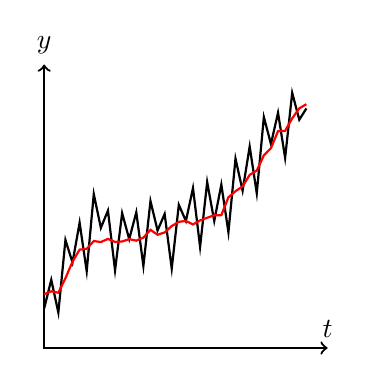
\begin{tikzpicture}[scale=0.18]
				% \draw [step=1, gray, very thin] (0, 0) grid (20, 20);
				\draw [thick, <->] (0, 20) node [anchor=south] {$y$} -- (0, 0) -- (20, 0) node [anchor=south] {$t$};
				\draw [thick, black] 
				(0.0, 2.794) -- (0.5, 4.810) -- 
				(1.0, 2.500) -- (1.5, 7.619) -- 
				(2.0, 6.031) -- (2.5, 8.840) -- 
				(3.0, 5.420) -- (3.5, 10.855) -- 
				(4.0, 8.474) -- (4.5, 9.695) -- 
				(5.0, 5.481) -- (5.5, 9.512) -- 
				(6.0, 7.680) -- (6.5, 9.573) -- 
				(7.0, 5.787) -- (7.5, 10.366) -- 
				(8.0, 8.291) -- (8.5, 9.451) -- 
				(9.0, 5.604) -- (9.5, 10.099) -- 
				(10.0, 8.962) -- (10.5, 11.282) -- 
				(11.0, 7.130) -- (11.5, 11.709) -- 
				(12.0, 8.962) -- (12.5, 11.526) -- 
				(13.0, 8.168) -- (13.5, 13.358) -- 
				(14.0, 11.099) -- (14.5, 14.213) -- 
				(15.0, 10.916) -- (15.5, 16.290) -- 
				(16.0, 14.396) -- (16.5, 16.595) -- 
				(17.0, 13.419) -- (17.5, 18.000) -- 
				(18.0, 16.106) -- (18.5, 16.900); 
				\draw [thick, red] 
				(0.0, 3.7939) -- (0.5, 3.9982) -- 
				(1.0, 3.9000) -- (1.5, 4.9183) -- 
				(2.0, 6.0905) -- (2.5, 6.9397) -- 
				(3.0, 6.9998) -- (3.5, 7.5450) -- 
				(4.0, 7.4733) -- (4.5, 7.6947) -- 
				(5.0, 7.4809) -- (5.5, 7.5115) -- 
				(6.0, 7.6794) -- (6.5, 7.5725) -- 
				(7.0, 7.7863) -- (7.5, 8.3336) -- 
				(8.0, 7.9901) -- (8.5, 8.1504) -- 
				(9.0, 8.6031) -- (9.5, 8.9008) -- 
				(10.0, 8.9618) -- (10.5, 8.7176) -- 
				(11.0, 8.9998) -- (11.5, 9.1901) -- 
				(12.0, 9.3618) -- (12.5, 9.3733) -- 
				(13.0, 10.6321) -- (13.5, 11.0588) --
				(14.0, 11.3992) -- (14.5, 12.2137) -- 
				(15.0, 12.5160) -- (15.5, 13.5901) -- 
				(16.0, 14.0969) -- (16.5, 15.2954) -- 
				(17.0, 15.3198) -- (17.5, 16.2000) -- 
				(18.0, 16.9069) -- (18.5, 17.2008);
			\end{tikzpicture}
		\end{multicols}
		
		\begin{itemize}[leftmargin=*]
			\item This problem is \textbf{spurious regression}. A seasonal adjustment can solve it.
		\end{itemize}
		
		A simple \textbf{seasonal adjustment} could be creating stationary binary variables and adding them to the model. For example, for quarterly series ($Q q_{t}$ are binary variables):
		
		\begin{center}
			$y_{t} = \beta_{0} + \beta_{1} Q2_{t} + \beta_{2} Q3_{t} + \beta_{3} Q4_{t} + \beta_{4} x_{1t} + \cdots + \beta_{k} x_{kt} + u_{t}$
		\end{center}
		
		Another way is to seasonally adjust (sa) the variables, and then, do the regression with the adjusted variables:
		
		\begin{center}
			$z_{t} = \beta_{0} + \beta_{1} Q2_{t} + \beta_{2} Q3_{t} + \beta_{3} Q4_{t} + v_{t} \rightarrow \hat{v}_{t} + \E(z_{t}) = \hat{z}_{t}^{sa}$
			
			$\hat{y}_{t}^{sa}= \beta_{0} + \beta_{1} \hat{x}_{1t}^{sa} + \cdots + \beta_{k} \hat{x}_{kt}^{sa} + u_{t}$
		\end{center}
		
		There are much better and complex methods to seasonally adjust a time series, like the \textbf{X-13ARIMA-SEATS}.
		
		\columnbreak
		
		\section*{Autocorrelation}
		
		The residual of any observation, $u_{t}$, is correlated with the residual of any other observation. The observations are not independent. Is the \textbf{non-fulfillment} of \textbf{t5}.
		
		\begin{center}
			$\Corr(u_{t}, u_{s} \mid x_{1}, \ldots, x_{k}) = \Corr(u_{t}, u_{s}) \neq 0, \; \forall t \neq s$
		\end{center}
		
		\subsection*{Consequences}
		
		\begin{itemize}[leftmargin=*]
			\item OLS estimators still are unbiased.
			\item OLS estimators still are consistent.
			\item OLS is \textbf{not efficient} anymore, but still a LUE (Linear Unbiased Estimator).
			\item \textbf{Variance estimations} of the estimators are \textbf{biased}: the construction of confidence intervals and the hypothesis testing is not reliable.
		\end{itemize}
		
		\subsection*{Detection}
		
		\begin{itemize}[leftmargin=*]
			\item \textbf{Scatter plots} - look for scatter patterns on $u_{t - 1}$ vs. $u_{t}$.
			
			\setlength{\multicolsep}{0pt}
			\setlength{\columnsep}{6pt}
			\begin{multicols}{3}
				\begin{center}
					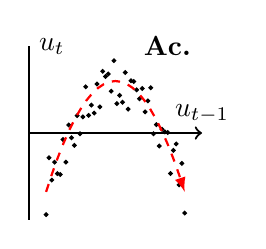
\begin{tikzpicture}[scale=0.11]
						\node at (16, 20) {\textbf{Ac.}}; 
						\draw [thick, ->] (0, 10) -- (20, 10) node [anchor=south] {$u_{t - 1}$}; 
						\draw [thick, -] (0, 0) -- (0, 20) node [anchor=west] {$u_{t}$}; 
						\draw plot [only marks, mark=*, mark size=6, domain=2:18, samples=50] (\x, {-0.2*(\x - 10)^2 + 13 + 6*rnd}); 
						\draw [thick, dashed, red, -latex] plot [domain=2:18] (\x, {-0.2*(\x - 10)^2 + 16});
					\end{tikzpicture}
				\end{center}
				
				\columnbreak
				
				\begin{center}
					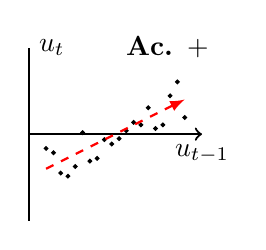
\begin{tikzpicture}[scale=0.11]
						\node at (16, 20) {\textbf{Ac. $+$}}; 
						\draw [thick, ->] (0, 10) -- (20, 10) node [anchor=north] {$u_{t - 1}$}; 
						\draw [thick, -] (0, 0) -- (0, 20) node [anchor=west] {$u_{t}$}; 
						\draw plot [only marks, mark=*, mark size=6, domain=2:18, samples=20] (\x, {5*rnd + 2.5 + 0.5*\x}); 
						\draw [thick, dashed, red, -latex] plot [domain=2:18] (\x, {5 + 0.5*\x});
					\end{tikzpicture}
				\end{center}
				
				\columnbreak
				
				\begin{center}
					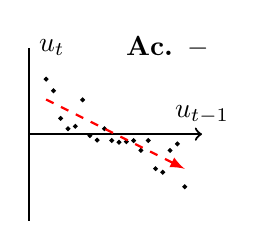
\begin{tikzpicture}[scale=0.11]
						\node at (16, 20) {\textbf{Ac. $-$}}; 
						\draw [thick, ->] (0, 10) -- (20, 10) node [anchor=south] {$u_{t - 1}$}; 
						\draw [thick, -] (0, 0) -- (0, 20) node [anchor=west] {$u_{t}$}; 
						\draw plot [only marks, mark=*, mark size=6, domain=2:18, samples=20] (\x, {5*rnd + 12.5 - 0.5*\x}); 
						\draw [thick, dashed, red, -latex] plot [domain=2:18] (\x, {15 - 0.5*\x});
					\end{tikzpicture}
				\end{center}
			\end{multicols}
			
			\begin{multicols}{2}
				\item \textbf{Correlogram} - autocorrelation function (ACF) and partial ACF (PACF).
				
				\columnbreak
				
				\begin{itemize}[leftmargin=*]
					\item Y axis: correlation.
					\item X axis: lag number.
					\item Grey area: $\pm 1.96/T^{0.5}$
				\end{itemize}
			\end{multicols}
			
			\begin{center}
				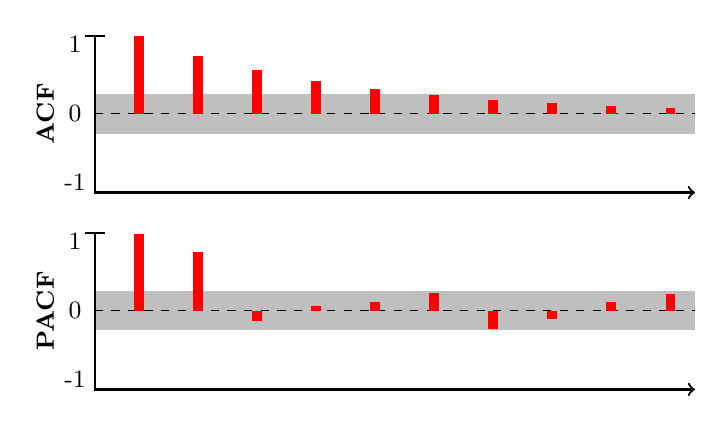
\begin{tikzpicture}[scale=0.25]
					% acf plot
					\node at (-2.5, 14) {\small \rotatebox{90}{\textbf{ACF}}}; 
					\node at (-1, 17.5) {\small 1};
					\node at (-1, 14) {\small 0};
					\node at (-1, 10.5) {\small -1}; 
					\fill [lightgray] (0, 13) rectangle (30.5, 15); 
					\draw [dashed, thin] (0, 14) -- (30.5, 14); 
					\draw [thick, |->] (0, 18) -- (0, 10) -- (30.5, 10);
					\fill [red] (2, 14) rectangle (2.5, 17.95);
					\fill [red] (5, 14) rectangle (5.5, 16.96);
					\fill [red] (8, 14) rectangle (8.5, 16.22); 
					\fill [red] (11, 14) rectangle (11.5, 15.67);
					\fill [red] (14, 14) rectangle (14.5, 15.25);
					\fill [red] (17, 14) rectangle (17.5, 14.94);
					\fill [red] (20, 14) rectangle (20.5, 14.70);
					\fill [red] (23, 14) rectangle (23.5, 14.53);
					\fill [red] (26, 14) rectangle (26.5, 14.40);
					\fill [red] (29, 14) rectangle (29.5, 14.30);
					% pacf plot
					\node at (-2.5, 4) {\small \rotatebox{90}{\textbf{PACF}}};
					\node at (-1, 7.5) {\small 1};
					\node at (-1, 4) {\small 0};
					\node at (-1, 0.5) {\small -1};
					\fill [lightgray] (0, 3) rectangle (30.5, 5);
					\draw [dashed, thin] (0, 4) -- (30.5, 4);
					\draw [thick, |->] (0, 8) -- (0, 0) -- (30.5, 0);
					\fill [red] (2, 4) rectangle (2.5, 7.90);
					\fill [red] (5, 4) rectangle (5.5, 7.00);
					\fill [red] (8, 4) rectangle (8.5, 3.47);
					\fill [red]	(11, 4) rectangle (11.5, 4.24);
					\fill [red] (14, 4) rectangle (14.5, 4.43);
					\fill [red] (17, 4) rectangle (17.5, 4.89);
					\fill [red] (20, 4) rectangle (20.5, 3.09);
					\fill [red] (23, 4) rectangle (23.5, 3.58);
					\fill [red] (26, 4) rectangle (26.5, 4.46);
					\fill [red] (29, 4) rectangle (29.5, 4.86);
				\end{tikzpicture}
			\end{center}
			
			\textbf{MA($q$) process}. \underline{ACF}: only the first $q$ coefficients are significant, the remaining are abruptly canceled. \underline{PACF}: attenuated exponential fast decay or sine waves.
			
			\textbf{AR($p$) process}. \underline{ACF}: attenuated exponential fast decay or sine waves. \underline{PACF}: only the first $p$ coefficients are significant, the remaining are abruptly canceled.
			
			\columnbreak
			
			\textbf{ARMA($p, q$) process}. \underline{ACF} and \underline{PACF}: the coefficients are not abruptly canceled and presents a fast decay.

			If the ACF coefficients do not decay rapidly, there is a clear indicator of lack of stationarity in mean.
			
			\item \textbf{Formal tests} - Generally, $H_{0}$: No autocorrelation.
			
			Supposing that $u_{t}$ follows an AR(1) process:
			
			\begin{center}
				$u_{t} = \rho_{1} u_{t - 1} + \varepsilon_{t}$
			\end{center}
			
			where $\varepsilon_{t}$ is white noise.

			\textbf{AR(1) t test} (exogenous regressors):

			\begin{center}
				$t = \dfrac{\hat{\rho}_{1}}{\se(\hat{\rho}_{1})} \sim t_{T - k - 1, \alpha/2}$
			\end{center}

			\begin{itemize}[leftmargin=*]
				\item $H_{1}$: Autocorrelation of order one, AR(1).
			\end{itemize}

			\textbf{Durbin-Watson statistic} (exogenous regressors and residual normality):

			\begin{center}
				$d = \dfrac{\sum_{t=2}^{n} (\hat{u}_{t} - \hat{u}_{t - 1})^{2}}{\sum_{t=1}^{n} \hat{u}_{t}^{2}} \approx 2 \cdot (1 - \hat{\rho}_{1})$
			\end{center}
			
			Where $0 \leq d \leq 4$
			
			\begin{itemize}[leftmargin=*]
				\item $H_{1}$: Autocorrelation of order one, AR(1).
			\end{itemize}
			
			\begin{center}
				\begin{tabular}{ c | c | c | c }
					$d =$          & 0 & 2 & 4  \\ \hline
					$\rho \approx$ & 1 & 0 & -1
				\end{tabular}
				
				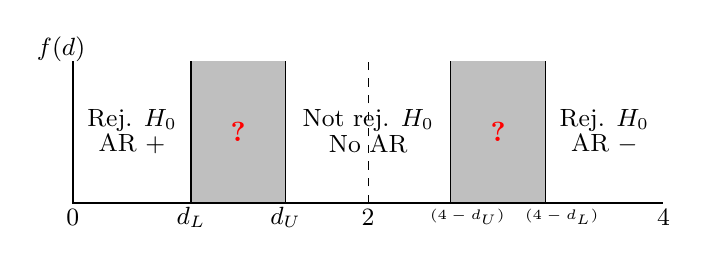
\begin{tikzpicture}[scale=0.3]
					\fill [lightgray] (5, 0) rectangle (9, 6); 
					\draw (5, 0) -- (5, 6);
					\draw (9, 0) -- (9, 6);
					\fill [lightgray] (16, 0) rectangle (20, 6);
					\draw (16, 0) -- (16, 6);
					\draw (20, 0) -- (20, 6);
					\draw [thick] (0, 6) -- (0, 0) -- (25, 0);
					\draw [dashed] (12.5, 0) -- (12.5, 6);
					\node at (-0.5, 6.5) {\small $f(d)$};
					\node at (0, -0.6) {\small 0};
					\node at (5, -0.6) {\small $d_{L}$};
					\node at (9, -0.6) {\small $d_{U}$};
					\node at (12.5, -0.6) {\small 2};
					\node at (16.7, -0.6) {\tiny $(4 - d_{U})$};
					\node at (20.7, -0.6) {\tiny $(4 - d_{L})$};
					\node at (25, -0.6) {\small 4};
					\node at (2.5, 3.5) {\small Rej. $H_{0}$};
					\node at (2.5, 2.5) {\small AR $+$};
					\node [text=red] at (7, 3) {\textbf{?}};
					\node at (12.5, 3.5) {\small Not rej. $H_{0}$};
					\node at (12.5, 2.5) {\small No AR};
					\node [text=red] at (18, 3) {\textbf{?}};
					\node at (22.5, 3.5) {\small Rej. $H_{0}$};
					\node at (22.5, 2.5) {\small AR $-$};
				\end{tikzpicture}
			\end{center}
			
			\textbf{Durbin's h} (endogenous regressors):
			
			\begin{center}
				$h = \hat{\rho} \cdot \sqrt{\dfrac{T}{1 - T \cdot \upsilon}}$
			\end{center}
			
			where $\upsilon$ is the estimated variance of the coefficient associated to the endogenous variable.
			
			\begin{itemize}[leftmargin=*]
				\item $H_{1}$: Autocorrelation of order one, AR(1).
			\end{itemize}
			
			\textbf{Breusch-Godfrey test} (endogenous regressors): it can detect MA($q$) and AR($p$) processes ($\varepsilon_{t}$ is w. noise):
			
			\begin{itemize}[leftmargin=*]
				\item MA($q$): $u_{t} = \varepsilon_{t} - m_{1} u_{t - 1} - \cdots - m_{q} u_{t - q}$
				\item AR($p$): $u_{t} = \rho_{1} u_{t - 1} + \cdots + \rho_{p} u_{t - p}+ \varepsilon_{t}$
			\end{itemize}
			
			Under $H_{0}$: No autocorrelation:
			
			\begin{center}
				$\hfill T \cdot R^{2}_{\hat{u}_t}\underset{a}{\sim}\chi^{2}_{q} \hfill \textbf{or} \hfill T \cdot R^{2}_{\hat{u}_t}\underset{a}{\sim}\chi^{2}_{p} \hfill$
			\end{center}
			
			\begin{itemize}[leftmargin=*]
				\item $H_{1}$: Autocorrelation of order $q$ (or $p$).
			\end{itemize}
			
			\textbf{Ljung-Box Q test}:
			
			\begin{itemize}[leftmargin=*]
				\item $H_{1}$: Autocorrelation up to lag $h$.
			\end{itemize}
			
		\end{itemize}
		
		\columnbreak
		
		\subsection*{Correction}
		
		\begin{itemize}[leftmargin=*]
			\item Use OLS with a variance-covariance matrix estimator that is \textbf{robust to heterocedasticity and autocorrelation} (HAC), for example, the one proposed by \textbf{Newey-West}.
			\item Use \textbf{Generalized Least Squares} (GLS). Supposing $y_{t} = \beta_{0} + \beta_{1} x_{t} + u_{t}$, with $u_{t} = \rho u_{t - 1}+ \varepsilon_{t}$, where $\lvert \rho \rvert < 1$ and $\varepsilon_{t}$ is \underline{white noise}.
			
			\begin{itemize}[leftmargin=*]
				\item If $\rho$ is \textbf{known}, use a \textbf{quasi-differentiated model}:
			
				\begin{center}
					$y_{t} - \rho y_{t - 1}= \beta_{0} (1 - \rho) + \beta_{1} (x_{t} - \rho x_{t - 1}) + u_{t} - \rho u_{t - 1}$
					
					$y_{t}^{*} = \beta_{0}^{*} + \beta_{1}' x_{t}^{*} + \varepsilon_{t}$
				\end{center}
				
				where $\beta_{1}' = \beta_{1}$; and estimate it by OLS.
				
				\item If $\rho$ is \textbf{not known}, estimate it by -for example- the \textbf{Cochrane-Orcutt iterative method} (Prais-Winsten method is also good):
				
				\begin{enumerate}[leftmargin=*]
					\item Obtain $\hat{u}_{t}$ from the original model.
					\item Estimate $\hat{u}_{t} = \rho \hat{u}_{t-1} + \varepsilon_{t}$ and obtain $\hat{\rho}$.
					\item Create a quasi-differentiated model:
					
					\begin{center}
						$y_{t} - \hat{\rho}y_{t - 1} = \beta_{0} (1 - \hat{\rho}) + \beta_{1} (x_{t} - \hat{\rho} x_{t - 1}) + u_{t} - \hat{\rho}u_{t - 1}$
						
						$y_{t}^{*} = \beta_{0}^{*} + \beta_{1}' x_{t}^{*} + \varepsilon_{t}$
					\end{center}
					
					where $\beta_{1}' = \beta_{1}$; and estimate it by OLS.
					
					\item Obtain $\hat{u}_{t}^{*} = y_{t} - (\hat{\beta}_{0}^{*} + \hat{\beta}_{1}' x_{t}) \neq y_{t} - (\hat{\beta}_{0}^{*} + \hat{\beta}_{1}' x_{t}^{*})$.
					\item Repeat from step 2. The algorithm ends when the estimated parameters vary very little between iterations.
				\end{enumerate}
			\end{itemize}
			
			\item If not solved, look for \textbf{high dependence} in the series.
		\end{itemize}
		
		\section*{Exponential smoothing}
		
		\begin{center}
			$f_{t} = \alpha y_{t} + (1 - \alpha) f_{t - 1}$
		\end{center}
		
		where $0 < \alpha < 1$ is the smoothing parameter.
		
		\section*{Predictions}
		
		Two types of predictions:
		
		\begin{itemize}[leftmargin=*]
			\item Of the mean value of $y$ for a specific value of $x$.
			\item Of an individual value of $y$ for a specific value of $x$.
		\end{itemize}
		
		\textbf{Theil's U statistic} - compares the forecasted results with the results of forecasting with minimal historical data.
		
		\begin{center}
			$U = \sqrt{\frac{\sum_{t=1}^{T-1} \left( \frac{\hat{y}_{t+1} - y_{t+1}}{y_t} \right)^2}{\sum_{t=1}^{T-1} \left( \frac{y_{t+1} - y_t}{y_t} \right)^2}}$
		\end{center}
		
		\begin{itemize}[leftmargin=*]
			\item $< 1$: The forecast is better than guessing.
			\item $= 1$: The forecast is about as good as guessing.
			\item $> 1$: The forecast is worse than guessing.
		\end{itemize}
		
		\columnbreak
		
		\section*{Stationarity}
		
		Stationarity allows to correctly identify relations --that stay unchanged with time-- between variables.
		
		\begin{itemize}[leftmargin=*]
			\item \textbf{Stationary process} (strict stationarity) - if any collection of random variables is taken and shifted $h$ periods (time changes), the joint probability distribution should stay unchanged.
			\item \textbf{Non-stationary process} - for example, a series with trend, where at least the mean changes with time.
			\item \textbf{Covariance stationary process} - its a weaker form of stationarity:
			
			\begin{itemize}[leftmargin=*]
				\begin{multicols}{2}
					\item $\E(x_{t})$ is constant.
					
					\columnbreak
					
					\item $\Var(x_{t})$ is constant.
				\end{multicols}
				
				\item For any $t$, $h \geq 1$, the $\Cov(x_{t}, x_{t + h})$ depends only of $h$, not of $t$.
			\end{itemize}
		\end{itemize}
		
		\section*{Weak dependence}
		
		Weak dependence replaces the random sampling assumption for time series.
		
		\begin{itemize}[leftmargin=*]
			\item An stationary process $\lbrace x_{t} \rbrace$ is \textbf{weakly dependent} when $x_{t}$ and $x_{t + h}$ are almost independent as $h$ increases without a limit.
			\item A covariance stationary process is \textbf{weakly dependent} if the correlation between $x_{t}$ and $x_{t + h}$ tends to $0$ fast enough when $h \rightarrow \infty$ (they are not asymptotically correlated).
		\end{itemize}
		
		Weakly dependent processes are known as \textbf{integrated of order zero}, I(0). Some examples:
		
		\begin{itemize}[leftmargin=*]
			\item \textbf{Moving average} - $\lbrace x_{t} \rbrace$ is a moving average of order $q$, MA($q$):
			
			\begin{center}
				$x_{t} = e_{t} + m_{1} e_{t - 1} + \cdots + m_{q} e_{t - q}$
			\end{center}
			
			where $\lbrace e_{t} : t = 0, 1, \ldots, T \rbrace$ is an \textsl{i.i.d.} sequence with zero mean and $\sigma^{2}_{e}$ variance.
			
			\item \textbf{Autoregressive process} - $\lbrace x_{t} \rbrace$ is an autoregressive process of order $p$, AR($p$):
			
			\begin{center}
				$x_{t} = \rho_{1} x_{t - 1} + \cdots + \rho_{p} x_{t - p} + e_{t}$
			\end{center}
			
			where $\lbrace e_{t} : t = 1, 2, \ldots, T \rbrace$ is an \textsl{i.i.d.} sequence with zero mean and $\sigma^{2}_{e}$ variance.
			
			\textbf{Stability condition}: if $1 - \rho_{1} z - \cdots - \rho_{p} z^{p} = 0$ for $\lvert z \rvert > 1$ then $\lbrace x_{t} \rbrace$ is an AR($p$) stable process that is weakly dependent. For AR(1), the condition is: $\lvert \rho_{1} \rvert < 1$.
		
			\item \textbf{ARMA process} - is a combination of AR($p$) and MA($q$); $\lbrace x_{t} \rbrace$ is an ARMA($p, q$):
			
			\begin{center}
				$x_{t} = e_{t} + m_{1} e_{t - 1} + \cdots + m_{q} e_{t - q} + \rho_{1} x_{t - 1} + \cdots + \rho_{p} x_{t - p}$
			\end{center}
		\end{itemize}
		
		\columnbreak
		
		\section*{Unit roots}
		
		A process is I($d$), that is, integrated of order $d$, if applying differences $d$ times makes the process stationary.
		
		When $d \geq 1$, the process is called a \textbf{unit root process} or it is said to have an unit root.
		
		A process have an unit root when the stability condition is not met (there are roots on the unit circle).
		
		\subsection*{Strong dependence}
		
		Most of the time, economics series are strongly dependent (or high persistent). Some examples of \textbf{unit root} I(1):
		
		\begin{itemize}[leftmargin=*]
			\item \textbf{Random walk} - an AR(1) process with $\rho_{1} = 1$.
			
			\begin{center}
				$y_{t} = y_{t - 1} + e_{t}$
			\end{center}
			
			where $\lbrace e_{t} : t = 1, 2, \ldots, T \rbrace$ is an \textsl{i.i.d.} sequence with zero mean and $\sigma^{2}_{e}$ variance.
			
			\item \textbf{Random walk with a drift} - an AR(1) process with $\rho_{1} = 1$ and a constant.
			
			\begin{center}
				$y_{t} = \beta_{0} + y_{t - 1} + e_{t}$
			\end{center}
			
			where $\lbrace e_{t} : t = 1, 2, \ldots, T \rbrace$ is an \textsl{i.i.d.} sequence with zero mean and $\sigma^{2}_{e}$ variance.
		\end{itemize}
		
		\subsection*{Unit root tests}
		
		\begin{center}
			\begin{tabular}{ c | c | c }
				Test            & $H_{0}$    & Reject $H_{0}$                     \\ \hline
				ADF             & I(1)       & tau \textless \, Critical value    \\ \hline
				KPSS            & I(0) level & mu \textgreater \, Critical value  \\
				                & I(0) trend & tau \textgreater \, Critical value \\ \hline
				Phillips-Perron & I(1)       & Z-tau \textless \, Critical value  \\ \hline
				Zivot-Andrews   & I(1)       & tau \textless \, Critical value
			\end{tabular}
		\end{center}
		
		\subsection*{From unit root to weak dependence}
		
		Integrated of \textbf{order one}, I(1), means that \textbf{the first difference} of the process is \textbf{weakly dependent} or I(0) (and usually, stationary). For example, let $\lbrace y_{t} \rbrace$ be a random walk:
		
		\begin{multicols}{2}
			\begin{center}
				$\Delta y_{t} = y_{t} - y_{t - 1} = e_{t}$
			\end{center}
			
			where $\lbrace e_{t} \rbrace = \lbrace \Delta y_{t} \rbrace$ is \textsl{i.i.d.} \\

			Note:
			\begin{itemize}[leftmargin=*]
				\item The first difference of a series removes its trend.
				\item Logarithms of a series stabilizes its variance.
			\end{itemize}
			
			\columnbreak
			
			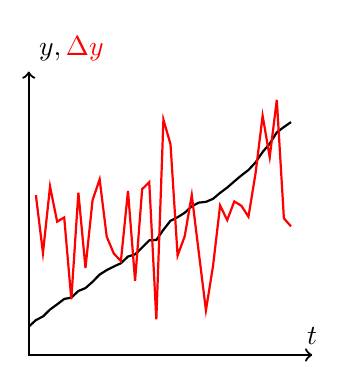
\begin{tikzpicture}[scale=0.18]
				% \draw [step=1, gray, very thin] (0, 0) grid (20, 20); 
				\draw [thick, <->] (0, 20) node [anchor=south west] {$y, {\color{red} \Delta y}$} -- (0, 0) -- (20, 0) node [anchor=south] {$t$}; 
				\draw [thick, black] 
				(0.0, 2.000) -- (0.5, 2.459) -- 
				(1.0, 2.716) -- (1.5, 3.205) -- 
				(2.0, 3.571) -- (2.5, 3.952) -- 
				(3.0, 4.047) -- (3.5, 4.514) -- 
				(4.0, 4.719) -- (4.5, 5.160) -- 
				(5.0, 5.674) -- (5.5, 5.987) -- 
				(6.0, 6.242) -- (6.5, 6.471) -- 
				(7.0, 6.944) -- (7.5, 7.104) -- 
				(8.0, 7.584) -- (8.5, 8.087) -- 
				(9.0, 8.112) -- (9.5, 8.834) -- 
				(10.0, 9.470) -- (10.5, 9.718) -- 
				(11.0, 10.032) -- (11.5, 10.491) -- 
				(12.0, 10.748) -- (12.5, 10.805) -- 
				(13.0, 11.016) -- (13.5, 11.439) --
				(14.0, 11.810) -- (14.5, 12.247) -- 
				(15.0, 12.668) -- (15.5, 13.052) -- 
				(16.0, 13.586) -- (16.5, 14.322) -- 
				(17.0, 14.913) -- (17.5, 15.704) -- 
				(18.0, 16.081) -- (18.5, 16.431); 
				\draw [thick, red] 
				(0.5, 11.283) -- (1.0, 7.201) -- 
				(1.5, 11.889) -- (2.0, 9.405) -- 
				(2.5, 9.701) -- (3.0, 3.926) -- 
				(3.5, 11.454) -- (4.0, 6.136) -- 
				(4.5, 10.926) -- (5.0, 12.393) -- 
				(5.5, 8.345) -- (6.0, 7.157) -- 
				(6.5, 6.627) -- (7.0, 11.572) -- 
				(7.5, 5.235) -- (8.0, 11.703) -- 
				(8.5, 12.186) -- (9.0, 2.513) -- 
				(9.5, 16.607) -- (10.0, 14.869) -- 
				(10.5, 7.015) -- (11.0, 8.368) -- 
				(11.5, 11.283) -- (12.0, 7.196) -- 
				(12.5, 3.153) -- (13.0, 6.277) -- 
				(13.5, 10.547) -- (14.0, 9.517) -- 
				(14.5, 10.834) -- (15.0, 10.526) -- 
				(15.5, 9.754) -- (16.0, 12.816) -- 
				(16.5, 16.875) -- (17.0, 13.961) -- 
				(17.5, 18.000) -- (18.0, 9.644) -- 
				(18.5, 9.075);
			\end{tikzpicture}
		\end{multicols}
		
		\columnbreak
		
		\subsubsection*{From unit root to percentage change}
		
		When an I(1) series is strictly positive, it is usually converted to logarithms before taking the first difference to obtain the (approx.) percentage change of the series:
		
		\begin{center}
			$\Delta \log(y_{t}) = \log(y_{t}) - \log(y_{t - 1}) \approx \dfrac{y_t - y_{t - 1}} {y_{t - 1}}$
		\end{center}
		
		\section*{Cointegration}
		
		When \textbf{two series are I(1), but a linear combination of them is I(0)}. If the case, the regression of one series over the other is not spurious, but expresses something about the long term relation. Variables are called cointegrated if they have a common stochastic trend.
		
		For example, $\lbrace x_{t} \rbrace$ and $\lbrace y_{t} \rbrace$ are I(1), but $y_{t} - \beta x_{t} = u_{t}$ where $\lbrace u_{t} \rbrace$ is I(0). ($\beta$ is the cointegrating parameter).

		\subsection*{Cointegration test}
		
		Following the example above:
		
		\begin{enumerate}[leftmargin=*]
			\item Estimate $y_{t} = \alpha + \beta x_{t} + \varepsilon_{t}$ and obtain $\hat{\varepsilon}_{t}$.
			\item Perform an ADF test on $\hat{\varepsilon}_{t}$ with a modified distribution.
			
			The result of this test is equivalent to:
			
			\begin{itemize}[leftmargin=*]
				\item $H_{0}$: $\beta = 0$ (no cointegration)
				\item $H_{1}$: $\beta \neq 0$ (cointegration)
			\end{itemize}
			
			if test statistic $>$ critical value, reject $H_0$.
		\end{enumerate}

		\section*{Heterocedasticity on time series}
		
		The \textbf{assumption} affected is \textbf{t4}, which leads \textbf{OLS to be not efficient}.
		
		Use tests like Breusch-Pagan or White's, where $H_{0}$: No heterocedasticity. It is \textbf{important} for the tests to work that there is \textbf{no autocorrelation}.
		
		\subsection*{ARCH}
		
		An autoregressive conditional heterocedasticity (ARCH), is a model to analyze a form of dynamic heterocedasticity, where the error variance follows an AR($p$) process.
		
		Given the model: $y_{t} = \beta_{0} + \beta_{1} z_{t} + u_{t}$ where, there is AR(1) and heterocedasticity:
		
		\begin{center}
			$\E(u^{2}_{t} \mid u_{t - 1}) = \alpha_{0} + \alpha_{1} u^{2}_{t - 1}$
		\end{center}
		
		\subsection*{GARCH}
		
		A general autoregressive conditional heterocedasticity (GARCH), is a model similar to ARCH, but in this case, the error variance follows an ARMA($p, q$) process.
	\end{multicols}
\end{document}